\documentclass{../UTNetLab}

\title{Multicast and Realtime Service}
\newcommand\reference{
   S. Panwar, S. Mao, J.-dong Ryoo, and Y. Li, “Multicast and realtime service,” in TCP/IP Essentials: A Lab-Based Approach, Cambridge: Cambridge University Press, 2004, pp. 134–158.
}

\begin{document}
\part{Simple Multicast Exercises\label{sec:simple-multicast}}
    For all the exercises in this section, the network topology is given in \hyperref[fig:1.3]{Figure~1.3}, where all the hosts are connected to a single network segment using their default IP addresses, i.e.\ from 128.238.66.100 to 128.238.66.107.
    
    \begin{minipage}{0.48\textwidth}
        \begin{flushleft}
            \begin{table}[H]
                \caption{The IP addresses of the hosts (Table~1.2)}
                \label{tab:1.2}
                \centering
                \begin{tabular}{ c c c }
                    \hline \hline
                    Host & IP Address & Subnet Mask \\
                    \hline 
                    h0 & 128.238.66.100 & 255.255.255.0 \\
                    h1 & 128.238.66.101 & 255.255.255.0 \\
                    h2 & 128.238.66.102 & 255.255.255.0 \\
                    h3 & 128.238.66.103 & 255.255.255.0 \\
                    h4 & 128.238.66.104 & 255.255.255.0 \\
                    h5 & 128.238.66.105 & 255.255.255.0 \\
                    h6 & 128.238.66.106 & 255.255.255.0 \\
                    h7 & 128.238.66.107 & 255.255.255.0 \\
                    \hline \hline
                    \end{tabular}
            \end{table}
        \end{flushleft}
    \end{minipage}
    \begin{minipage}{0.48\textwidth}
        \begin{flushright}
            \begin{figure}[H]
                \centering
                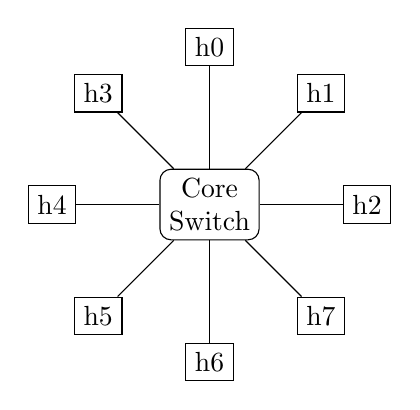
\begin{tikzpicture}
                    \node[draw,rounded corners,align=center] (s) at (0,0) {Core\\Switch};
                    \node[draw] (h0) at (0,2){h0};
                    \node[draw] (h1) at ({sqrt(2)},{sqrt(2)}){h1};
                    \node[draw] (h2) at (2,0){h2};
                    \node[draw] (h3) at (-{sqrt(2)},{sqrt(2)}){h3};
                    \node[draw] (h4) at (-2,0){h4};
                    \node[draw] (h5) at (-{sqrt(2)},-{sqrt(2)}){h5};
                    \node[draw] (h6) at (0,-2){h6};
                    \node[draw] (h7) at ({sqrt(2)},-{sqrt(2)}){h7};
                
                    \draw (h0) -- (s);
                    \draw (h1) -- (s);
                    \draw (h2) -- (s);
                    \draw (h3) -- (s);
                    \draw (h4) -- (s);
                    \draw (h5) -- (s);
                    \draw (h6) -- (s);
                    \draw (h7) -- (s);
                \end{tikzpicture}
                \caption{A single segment network (Figure~1.3)}
                \label{fig:1.3}
            \end{figure}
        \end{flushright}
    \end{minipage}

    Launch GNS3 and make a network as above.

    To use prepared topology to GNS3:
    \begin{enumerate}
        \item Open \texttt{File} menu
        \item Select \texttt{Import }
        \begin{figure}[H]
            \centering
            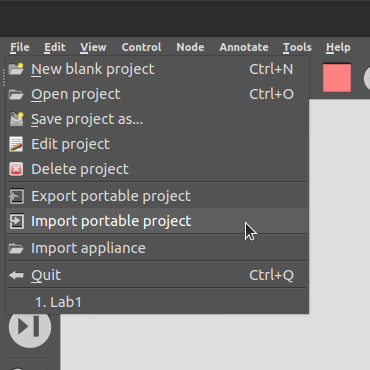
\includegraphics[scale=1.6]{img/import-1}
        \end{figure}
        \item Choose the figure from \texttt{Figures} folder
        \item Enter a name for new project
        \begin{figure}[H]
            \centering
            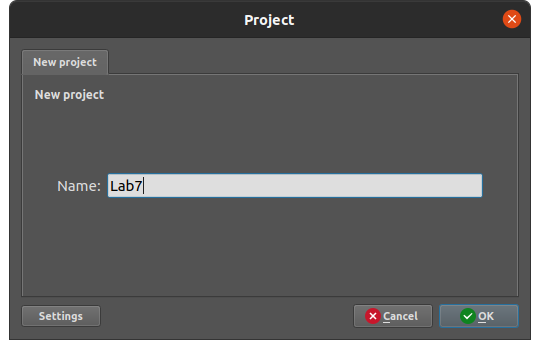
\includegraphics[scale=1.6]{img/import-2}
        \end{figure}
    \end{enumerate}

    After that, start all devices by clicking on the \texttt{Start/Resume all nodes} (green triangular button).
    \begin{figure}[H]
        \centering
        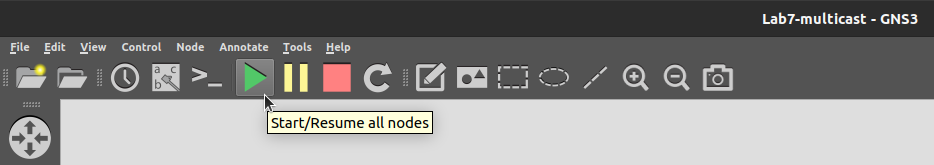
\includegraphics[scale=1.6]{img/start-all}
    \end{figure}

    To open a console, double click on a already-started machine.

%     Use a command like this to allocate IP address to each machine:
%     \begin{lstlisting}[emph=eth0]
% ifconfig eth0 128.238.66.100 netmask 255.255.255.0
%     \end{lstlisting}

\section{Linux Multicast Routing Table\label{sec:rt}}
\label{sec:linux-multicast-routing}
    Execute the following command to display the routing table of one host (for example \textit{h0}).
    \begin{lstlisting}
netstat -rn
    \end{lstlisting}
    
    If there is no entry for the 224.0.0.0 subnet, you need to provide a default route for multicast traffic, by:
    \footnote{This command can be appended to the \path{/etc/rc.local} file, so that it will be executed automatically when the system bootstraps. Each time when the network interface is brought down and up again by the \lstinline{ifconfig} command, you may need to run the \lstinline{route} command to re-insert the multicast routing entry.}
    \begin{lstlisting}[emph=eth0]
route add -net 224.0.0.0 netmask 240.0.0.0 dev eth0
    \end{lstlisting}
    
    Execute this command on all hosts.
    Save the new routing table.
    
    \begin{report}
    \item Submit the routing table you saved.
    \end{report}

\section{Multicast Membership}
    Execute the following command to show the multicast group memberships for all the interfaces in your host (for example \textit{h0}).
    \begin{lstlisting}
netstat -g
    \end{lstlisting}
    
    \begin{report}
    \item How many multicast groups did the interface belong to? What were the groups? Explain the meaning of the group IDs.
    \end{report}

\section{Multicast \texttt{ping}}
    Set hosts \textit{h0}, \textit{h2}, \textit{h4} and \textit{h6} to replry linux multicast routing in all the hosts:
    \begin{lstlisting}[emph={eth0}]
echo 0 > /proc/sys/net/ipv4/icmp_echo_ignore_broadcasts
    \end{lstlisting}

    Execute following command on \textit{h1}:
    \begin{lstlisting}
ping 224.0.0.1
    \end{lstlisting}
    Examine the \lstinline{ping} output to see which hosts reply.

    Ping a broadcast address using:
    \begin{lstlisting}
ping -b 128.238.66.255
    \end{lstlisting}
    Examine the \lstinline{ping} output to see which hosts reply.

    % You can enable broadcast ping replay by: \lstinline{echo 0 > /proc/sys/net/ipv4/icmp_echo_ignore_broadcasts}.
    
    \begin{report}
    \item Which hosts replied when the multicast address was pinged?
    Which hosts replied when the broadcast address was pinged?

    \item In each case, was there a reply from your host?
    What if you ping from \textit{h0}?
    \end{report}

\section{Multicast vs Unicast\label{sec:multicast-vs-unicast}}
    On \textit{h1} execute \lstinline{tcpdump -n -nn -e} and \lstinline{tcpdump ether multicast -n -nn -e} (or run \lstinline{wireshark}) to capture an Ethernet unicast frame, an Ethernet multicast frame, and an Ethernet broadcast frame.

    You can open an auxiliary terminal by right-clicking on a host and selecting \texttt{Auxiliary console} if needed.
    \begin{figure}[H]
        \centering
        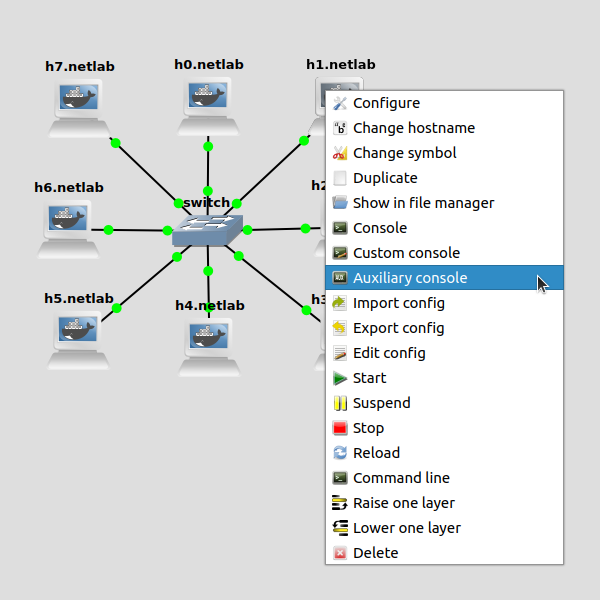
\includegraphics[scale=1.6]{img/auxiliary}
    \end{figure}

    Also, to open \lstinline{wireshark}, right-click on the link between host and switch and select \texttt{Start capture}.
    \begin{figure}[H]
        \centering
        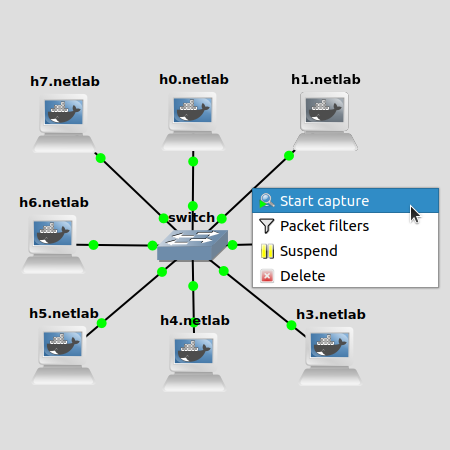
\includegraphics[scale=1.6]{img/capture}
    \end{figure}

    Execute the following command in \textit{h0} to generate an Ethernet multicast frame:
    \begin{lstlisting}[emph={your-host, remote-host}]
socket -i -u -n1 230.11.111.10 2000
    \end{lstlisting}

    Generate another Ethernet multicast frame, but with a different group address of {232.139.111.10}.

    To generate an Ethernet broadcast frame, you may \lstinline{ping} a remote host from \textit{h0} that has no entry in the ARP table of your host, e.g.\ \textit{h5}.
    \footnote{You can see ARP table by \lstinline{arp -a} delete a cached ARP entry by \lstinline[emph={ip}]{arp -d ip}.}
    \begin{lstlisting}
ping 128.238.66.105
    \end{lstlisting}
    Recall that the ARP request is broadcast.%

    Save the frames captured for the lab report.

    \begin{report}
    \item Compare the source and destination MAC addresses of the frames you captured.

    \item Use one of the multicast frames captured to explain how a multicast group address is mapped to a multicast MAC address.

    For the two multicast frames captured, do they have the same destination MAC address?
    Why?
    \end{report}

\section{Simple UDP Multicast Client and Server}

    % \lstinline{netspy} and \lstinline{netspyd} programs are located in \textit{code} directory for \textit{netlab} user.
    
%     You can go there by the following command:
%     \begin{lstlisting}
% cd /home/netlab/code
%     \end{lstlisting}
    
%     You can compile source codes, if needed, by:
%     \begin{lstlisting}[emph={fileName, outputName}]
% gcc fileName -o outputName
%     \end{lstlisting}

    Start the multicast client \lstinline{netspy} on hosts \textit{h0}, \textit{h2}, \textit{h4} and \textit{h6}, by executing:%
    \footnote{If you get \textit{Netspy : cannot join multicast group `224.111.111.111'}, add route for the groups as described in \autoref{sec:rt}.}
    \begin{lstlisting}
/home/netlab/code/netspy 224.111.111.111 1500
    \end{lstlisting}
    
    Then, start the multicast sender \lstinline{netspyd} on \textit{h0}, by executing:
    \begin{lstlisting}
/home/netlab/code/netspyd 224.111.111.111 1500 1
    \end{lstlisting}
    You may need to open an auxiliary terminal as described in \autoref{sec:multicast-vs-unicast}.
    
    Execute \lstinline{tcpdump ip multicast} or \lstinline{wireshark} on every host to capture multicast IP datagrams.

%     Start \textit{ssh} service on \textit{h0} by:
%     \begin{lstlisting}
% service ssh start
%     \end{lstlisting}

    \lstinline{telnet} to \textit{h0} from a remote machine, e.g.\ \textit{h6}, using:
    \begin{lstlisting}
telnet 128.238.66.100
    \end{lstlisting}
    Use \texttt{netlab} as username and password.

    Save the captured multicast datagram sent by \lstinline{netspyd} and exit the \lstinline{telnet} session.

    \begin{report}
    \item From the \lstinline{tcpdump} output, how many messages are sent by \lstinline{netspyd} when a new user logged in to \textit{h0}?
    From the \lstinline{netspy} outputs on all the hosts, how many copies of the message are received in total?

    \item Did \textit{h0}, where the multicast sender, \lstinline{netspyd}, was running, receive the multicast datagram?
    Why?
    If yes, through which interface did \textit{h0} receive this datagram?
    \end{report}

\section{\texttt{ping} Replay}
    % Enable broadcast ping replay by: \lstinline{echo 0 > /proc/sys/net/ipv4/icmp_echo_ignore_broadcasts} on all hosts.
    Keep the \lstinline{netspy} and the \lstinline{tcpdump} (on \textit{h6}) programs running.
    Execute the following command from \textit{h6}:
    \begin{lstlisting}
ping 224.111.111.111
    \end{lstlisting}
    Examine the \lstinline{tcpdump} and \lstinline{ping} outputs to see which hosts replied.

    Terminate the \lstinline{netspy} programs on several hosts, e.g.\ \textit{h0} and \textit{h6}.
    Execute the \lstinline{ping} command again.

    Also, examine the \lstinline{tcpdump} and the \lstinline{ping} outputs (on \textit{h6}) to see which hosts replied.

    Ping a broadcast address using:
    \begin{lstlisting}
ping -b 128.238.66.255
    \end{lstlisting}
    Examine the \lstinline{ping} output to see which hosts reply and see the difference with multicast.


    \begin{report}
    \item Which hosts reply to \lstinline{ping} each time?
    \end{report}

\part{IGMP Exercises}\label{sec:igmp}
    In the following exercises, use four hosts and one router. The network topology is given in \hyperref[fig:7.13]{Figure~7.13}, and the corresponding host IP addresses and router IP addresses are given in \hyperref[tab:7.2]{Table~7.2} and \hyperref[tab:7.3]{Table~7.3}, respectively.

    \begin{table}[H]
        \caption{Hosts IP addresses for \hyperref[fig:7.13]{Figure~7.13} (Table~7.2)}
        \label{tab:7.2}
        \centering
        \begin{tabular}{ *3c }
            \hline \hline
            Name & IP Address \\
            \hline
                h1 & 128.238.63.101/24 \\
                h2 & 128.238.63.102/24 \\
                h3 & 128.238.64.103/24 \\
                h4 & 128.238.64.104/24 \\
            \hline \hline
            \end{tabular}
    \end{table}

    \begin{table}[H]
        \caption{Router IP addresses for \hyperref[fig:7.13]{Figure~7.13} (Table~7.3)}
        \label{tab:7.3}
        \centering
        \begin{tabular}{ *3c }
            \hline \hline
            Host & eth0 & eth1 \\
            \hline
            router & 128.238.63.3/24 & 128.238.64.3/24 \\
            \hline \hline
            \end{tabular}
    \end{table}

    \begin{figure}[H]
        \centering
        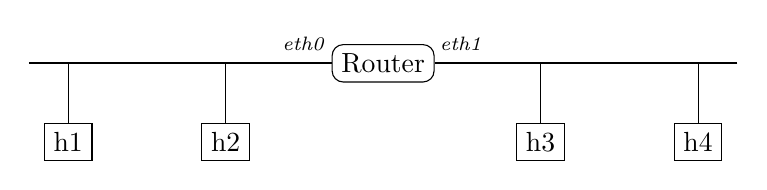
\begin{tikzpicture}
            \node[draw] (h1) at (-4,-1){h1};
            \node[draw] (h2) at (-2,-1){h2};
            \node[draw,rounded corners] (router) at (0,0){Router};
            \node[draw] (h3) at (2,-1){h3};
            \node[draw] (h4) at (4,-1){h4};
        
            \draw (h1) -- (-4,0);
            \draw (h2) -- (-2,0);
            \draw (h3) -- (2,0);
            \draw (h4) -- (4,0);
            \draw[thick] (4.5,0) -- (router);
            \draw[thick] (-4.5,0) -- (router);
            \draw (router) +(1,0.25) node[align=right] {\scriptsize\textit{eth1}};
            \draw (router) +(-1,0.25) node[align=left] {\scriptsize\textit{eth0}};
        \end{tikzpicture}
        \caption{The network topology for \nameref{sec:igmp} (Figure~7.13)}
        \label{fig:7.13}
    \end{figure}

    Enable linux multicast routing in all the hosts (see \autoref{sec:simple-multicast}):
    \begin{lstlisting}[emph={eth0}]
route add -net 224.0.0.0 netmask 240.0.0.0 dev eth0
route add -net 128.238.0.0/16 dev eth0
echo 0 > /proc/sys/net/ipv4/icmp_echo_ignore_broadcasts
    \end{lstlisting}

    You can use prepared topology as described in \autoref{sec:simple-multicast}.

\section{Configuring Router}
\label{sec:config-router}
    Connect the hosts and the route in your group as shown in \hyperref[fig:7.13]{Figure~7.13}.
    Set the IP address of your host as given in \hyperref[tab:7.2]{Table~7.2}.
    % Note that the IP addresses of the router interfaces are the same as their default IP addresses.
    Run \lstinline{ip multicast-routing} to enable multicast routing in the \textit{Global Configuration} mode.
    Then, enable the PIM protocol on each interface, by running \lstinline{ip pim dense-mode} in the \textit{Interface Configuration} mode.
    Now the router is enabled to do multicast routing using PIM.
    \begin{lstlisting}[language=cisco]
configure terminal
    ip multicast-routing
    interface f0/0
        ip address 128.238.63.3 255.255.255.0
        ip pim dense-mode
        no shutdown
        exit
    interface f0/1
        ip address 128.238.64.3 255.255.255.0
        ip pim dense-mode
        no shutdown
        exit
    end
    \end{lstlisting}

    Login to the router, execute the following commands in the \textit{Privileged EXEC} mode:
    \begin{lstlisting}[language=cisco]
show ip igmp interface
show ip igmp group
    \end{lstlisting}

    \begin{report}
    \item Examine the multicast group memberships currently recorded in the router and the configurations of the router interfaces.
    \end{report}

\section{Multicast Message}
    Enable linux multicast routing in all the hosts (see \autoref{sec:linux-multicast-routing}).\\
    Start \lstinline{netspy} on all the hosts, by using:
    \begin{lstlisting}
/home/netlab/code/netspy 224.111.111.111 1500
    \end{lstlisting}
    Start \lstinline{netspy} on \textit{h1}, by using:
    \begin{lstlisting}
/home/netlab/code/netspyd 224.111.111.111 1500 16
    \end{lstlisting}
    
    Login to the router.
    Run the following commands in the \textit{Privileged EXEC} mode again to examine the current membership records:
    \begin{lstlisting}[language=cisco]
show ip igmp interface
show ip igmp group
    \end{lstlisting}

    Can you \lstinline{ping} a host on the other side of the router (e.g.\ \lstinline{ping} \textit{h4} from \textit{h1})? If not, why not?
    \begin{lstlisting}
ping 128.238.64.104
    \end{lstlisting}

    \lstinline{telnet} from \textit{h2} to \textit{h1} in your group, then logout. (Use \texttt{netlab} as username and password.)
    \begin{lstlisting}
telnet 128.238.63.101
    \end{lstlisting}
    Does multicast messages sent by \lstinline{netspyd} reach the other side of the router? If not, why not?

    Add \textit{route} for \textbf{other subnet} to your host and try \lstinline{ping} again:
    \begin{lstlisting}[emph={eth0}]
route add -net 128.238.64.0/24 dev eth0  # on h1 & h2
route add -net 128.238.63.0/24 dev eth0  # on h3 & h4
    \end{lstlisting}
    Now, login to \textit{h1} from \textit{h2} in your group via \lstinline{telnet}, then logout.
    Check if multicast messages sent by \lstinline{netspyd} reach the other side of the router.
    
    \begin{report}
    \item Can you ping a host on the other side of the router?
    Will the router forward a multicast IP datagram to the other side?
    Justify your answers.
    \end{report}

\section{IGMP Types}
    Execute \lstinline{tcpdump} or \lstinline{wireshark}\footnote{If you have trouble in getting packets using \lstinline{wireshark}, try \lstinline{tcpdump}.} in one console to capture IGMP messages.
    \begin{lstlisting}[emph={eth0}]
tcpdump ip multicast -v
    \end{lstlisting}
    When you see \textbf{three or more IGMP queries} in the second \lstinline{tcpdump} output, terminate both \lstinline{tcpdump} programs.

    Analyze the IGMP messages you captured.
    Print and save two different IGMP messages.

    Repeat the above experiment.
    Terminate \lstinline{netspy} on \textit{h2} and \textit{h4}.
    Terminate the \lstinline{tcpdump} programs and analyze the IGMP leave message you captured.
    
    \begin{report}
    \item What is the value of the Time-to-Live (TTL) field for the IGMP messages?
    Why do we not set the TTL to a larger number?

    \item What is the default frequency at which the router sends IGMP queries?
    \end{report}

\section{Router Join to Multicast-Group}
    Login to the router.
    See if you can make a router interface (e.g.\ \textit{ethernet0}) join a multicast group of 224.0.0.2, using:
    \begin{lstlisting}[language={cisco}]
configure terminal
    ip multicast-routing
    interface f0/0
        ip igmp join-group 224.0.0.2
        exit
    end
    \end{lstlisting}
    
    \begin{report}
    \item Explain why the above command fails.
    \end{report}

\part{Multicast Routing Exercises\label{sec:multicast-routing}}
    For the rest of the exercises in this chapter, the network topology is given in \hyperref[fig:7.14]{Figure~7.14}. The IP addresses of the hosts and router interfaces are given in \hyperref[fig:7.14]{Figure~7.14}.
    \begin{figure}[H]
        \centering
        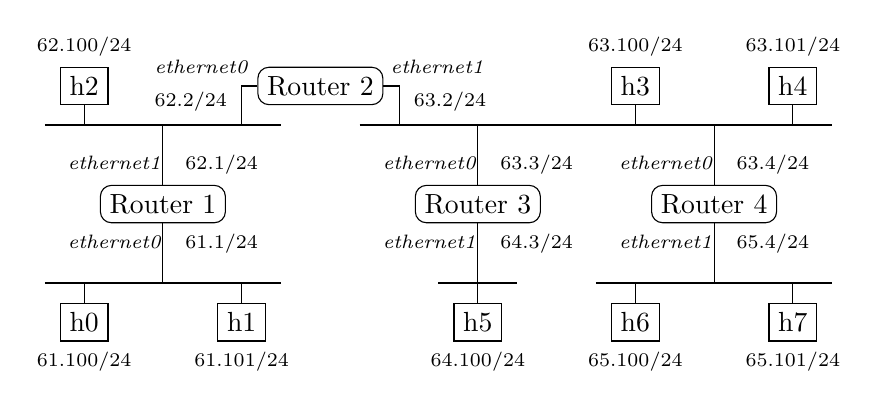
\begin{tikzpicture}
            \draw (0,0) node[draw,rounded corners,fill=white] (r1) {Router 1}
                (r1) -- +(0,1)
                (r1) -- +(0,-1)
                +(0,0.5) node {\scriptsize\textit{ethernet1}\quad 62.1/24}
                +(0,-0.5) node {\scriptsize\textit{ethernet0}\quad 61.1/24}
            ;
            \draw (2,1.5) node[draw,rounded corners,fill=white] (r2) {Router 2}
                (r2) -| +(1,-0.5)
                (r2) -| +(-1,-0.5)
                +(1.5,0) node[align=right] {\scriptsize\textit{ethernet1}\\\scriptsize63.2/24}
                +(-1.5,0) node[align=left] {\scriptsize\textit{ethernet0}\\\scriptsize62.2/24}
            ;
            \draw (4,0) node[draw,rounded corners,fill=white] (r3) {Router 3}
                (r3) -- +(0,1)
                (r3) -- +(0,-1)
                +(0,0.5) node {\scriptsize\textit{ethernet0}\quad 63.3/24}
                +(0,-0.5) node {\scriptsize\textit{ethernet1}\quad 64.3/24}
            ;
            \draw (7,0) node[draw,rounded corners,fill=white] (r4) {Router 4}
                (r4) -- +(0,1)
                (r4) -- +(0,-1)
                +(0,0.5) node {\scriptsize\textit{ethernet0}\quad 63.4/24}
                +(0,-0.5) node {\scriptsize\textit{ethernet1}\quad 65.4/24}
            ;
            \draw (-1,-1.5) node[draw,fill=white] (h0) {h0}
                -- +(0,0.5)
                +(0,-0.5) node {\scriptsize61.100/24}
            ;
            \draw (1,-1.5) node[draw,fill=white] (h1) {h1}
                -- +(0,0.5)
                +(0,-0.5) node {\scriptsize61.101/24}
            ;
            \draw (-1,1.5) node[draw,fill=white] (h2) {h2}
                -- +(0,-0.5)
                +(0,0.5) node {\scriptsize62.100/24}
            ;
            \draw (7-1,-1.5) node[draw,fill=white] (h6) {h6}
                -- +(0,0.5)
                +(0,-0.5) node {\scriptsize65.100/24}
            ;
            \draw (7+1,-1.5) node[draw,fill=white] (h7) {h7}
                -- +(0,0.5)
                +(0,-0.5) node {\scriptsize65.101/24}
            ;
            \draw (4,-1.5) node[draw,fill=white] (h5) {h5}
                -- +(0,0.5)
                +(0,-0.5) node {\scriptsize64.100/24}
            ;
            \draw (7-1,1.5) node[draw,fill=white] (h3) {h3}
                -- +(0,-0.5)
                +(0,0.5) node {\scriptsize63.100/24}
            ;
            \draw (7+1,1.5) node[draw,fill=white] (h4) {h4}
                -- +(0,-0.5)
                +(0,0.5) node {\scriptsize63.101/24}
            ;
            \draw[thick] (-1.5,-1) -- +(3,0);
            \draw[thick] (-1.5,1) -- +(3,0);
            \draw[thick] (4-1.5,1) -- +(6,0);
            \draw[thick] (4-0.5,-1) -- +(1,0);
            \draw[thick] (7-1.5,-1) -- +(3,0);
        \end{tikzpicture}
        \caption{The network topology for \nameref{sec:multicast-routing} (Figure~7.14)}
        \label{fig:7.14}
    \end{figure}

    You can use prepared topology as described in \autoref{sec:simple-multicast}.

\section{Multicast Multi-Hub\label{sec:multi-hub}}
    Enable linux multicast routing in all the hosts (see \autoref{sec:simple-multicast}):
    \begin{lstlisting}[emph={eth0}]
route add -net 224.0.0.0 netmask 240.0.0.0 dev eth0
route add -net 128.238.0.0/16 dev eth0
echo 0 > /proc/sys/net/ipv4/icmp_echo_ignore_broadcasts
    \end{lstlisting}

    Enable PIM multicast routing in all the routers (see \autoref{sec:config-router}). 
    \begin{lstlisting}[language={cisco}, emph={ethernet0_ip, ethernet1_ip}]
configure terminal
    ip multicast-routing
    interface f0/0
        ip address ethernet0_ip 255.255.255.0
        ip pim dense-mode
        no shutdown
        exit
    interface f0/1
        ip address ethernet1_ip 255.255.255.0
        ip pim dense-mode
        no shutdown
        exit
    end
    \end{lstlisting}

    Run \lstinline{tcpdump ip multicast} or \lstinline{wireshark} on all the hosts. 

    Execute \lstinline{netspy} client on \textit{h0}, \textit{h2}, \textit{h3}, \textit{h5}, and \textit{h6}:
    \begin{lstlisting}
/home/netlab/code/netspy 224.111.111.111 1500
    \end{lstlisting}

    Execute \lstinline{netspy} server on \textit{h4}:
    \begin{lstlisting}
/home/netlab/code/netspyd 224.111.111.111 1500 16
    \end{lstlisting}
    
    To generate multicast traffic, you can login (by \lstinline{telnet}) to or logout of \textit{h4} from \textit{h2}. (Use \texttt{netlab} as username and password.)
    \begin{lstlisting}
telnet 128.238.63.101
    \end{lstlisting}

    Each time when the login user set of \textit{h4} changes, \lstinline{netspyd} on \textit{h4} will send a multicast datagram to group 224.111.111.111, to report the change in its login users.

    Terminate the \lstinline{netspy} program on \textit{h6}.

    Save one of the PIM routing packets.
    You may use \lstinline{tcpdump} output to analyze it.
    
    \begin{report}
    \item While the \lstinline{netspy} program is running on \textit{h6},
    can you see the \lstinline{netspy} messages on the 128.238.65.0 (or the 128.238.61.0) subnet in the \lstinline{tcpdump} output?

    \item After terminating the \lstinline{netspy} program on \textit{h6},
    can you see the \lstinline{netspy} messages on the 128.238.65.0 (or the 128.238.61.0) subnet?%
    \footnote{If IGMPv1 is used, a participant does not send a leave message when it leaves the group.
    In this case, the membership record in the router expires in 120 seconds.
    During this interval, the router still forwards multicast datagram through the port.} 

    \item What is the destination IP address used in this PIM routing packet?
    \end{report}

\section{Multicast Tree}
    In this exercise, try the \lstinline[language={cisco}]{mstat} Cisco~IOS command to find the multicast tree from a source.
    The \lstinline[language={cisco}]{mstat} command is executable in the \textit{Privileged EXEC} mode.
    Its syntax is \lstinline[language={cisco}, emph={source, destination, group}]{mstat source [destination] [group]}, in which:
    \begin{description}
        \item[source] Specifies the IP address or name of the multicast source.
        \item[destination] (Optional) Specifies the IP address or name of the destination. If not provided, the router uses itself as the destination.
        \item[group] (Optional) Specifies the IP address or name of the group to display. The default is 224.2.0.1.
    \end{description}
    You can always type \lstinline[language={cisco}]{?} to get help on the syntax of the command.

    Keep \lstinline{netspy} running on hosts \textit{h0}, \textit{h2}, \textit{h3}, \textit{h5}, and \textit{h6} and server on \textit{h4} as described in \autoref{sec:multi-hub}.
    Try the following command in \textit{Router2}:
    \begin{lstlisting}[language={cisco}]
mstat 128.238.62.100 128.238.61.100 224.111.111.111
    \end{lstlisting}

    Generate multicast packet when execute command for specific source.

    \begin{report}
    \item Draw multicast tree from 128.238.62.100 to 128.238.61.100 via 224.111.111.111 group.
    \end{report}

\section{Multicast TTL}
    Keep \lstinline{netspy} running on hosts \textit{h0}, \textit{h2}, \textit{h3}, \textit{h5}, and \textit{h6} and server on \textit{h4} as described in \autoref{sec:multi-hub}.
    
    Ping the multicast group address from \textit{h4}, using: 
    \begin{lstlisting}[emph={n}]
ping 224.111.111.111 -t n
    \end{lstlisting}

    The parameter \textit{n} is the TTL to be set to the multicast datagrams sent by ping.
    Try different values of \textit{n}, e.g.\ 1, 2, 3, and 16.
    See how far a multicast datagram can travel with different TTL values. 

    Now, login to \textit{Router2}, in the \textit{Interface Configuration} mode, set the TTL threshold of the \textit{ethernet0} interface to 32, using:%
    \footnote{The syntax of this command may be different for different versions of Cisco~IOS. You may use \lstinline[language={cisco}]{?} to get help.}
    \begin{lstlisting}[language={cisco}]    
configure terminal
    interface f0/0
        ip multicast ttl-threshold 32
        exit
    end
    \end{lstlisting}

    Run the \lstinline{ping} command with $n = 16$ again.
    Can you see the multicast datagrams in the 128.238.61.0 and 128.238.62.0 subnet?
    Try $n = 33$.
    Answer the same question.
    
    \begin{report}
    \item At first, which hosts answered the \lstinline{ping} with \textit{n} equals to 1, 2, 3, and 16?
    \item After changing threshold of \textit{Router2} to 16, which hosts answered the \lstinline{ping} with \textit{n} equals to 16?
    Does datagrams reach 128.238.61.0 and 128.238.62.0 subnets?
    \item After changing threshold of \textit{Router2} to 16, which hosts answered the \lstinline{ping} with \textit{n} equals to 33?
    Does datagrams reach 128.238.61.0 and 128.238.62.0 subnets?
    
    \item What is the use of the TTL threshold in the router interface?
    \end{report}

\part{Multicast Video Streaming Exercise\label{sec:multicast-streaming}}
    In the following exercise, we use \lstinline{vlc} for video streaming.
    
    In the following exercises, use four hosts and one router. The network topology is given in \hyperref[fig:7.15]{Figure~7.15}\footnote{This figure is not in the book.}, and the corresponding host IP addresses and router IP addresses are given in \hyperref[tab:7.4]{Table~7.4} and \hyperref[tab:7.5]{Table~7.5}, respectively.
    Make sure you use a device with GUI (e.g.\ \texttt{utnetlab/gui}).

    \begin{table}[H]
        \caption{Hosts IP addresses for \hyperref[fig:7.15]{Figure~7.15} (Table~7.4)}
        \label{tab:7.4}
        \centering
        \begin{tabular}{ *3c }
            \hline \hline
            Name & IP Address \\
            \hline
                h0 & 128.238.61.100/24 \\
                h1 & 128.238.62.101/24 \\
                h2 & 128.238.62.102/24 \\
            \hline \hline
            \end{tabular}
    \end{table}

    \begin{table}[H]
        \caption{Router IP addresses for \hyperref[fig:7.15]{Figure~7.15} (Table~7.5)}
        \label{tab:7.5}
        \centering
        \begin{tabular}{ *3c }
            \hline \hline
            Host & eth0 & eth1 \\
            \hline
            router & 128.238.61.1/24 & 128.238.62.1/24 \\
            \hline \hline
            \end{tabular}
    \end{table}

    \begin{figure}[H]
        \centering
        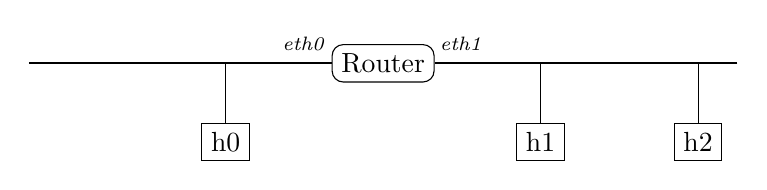
\begin{tikzpicture}
            \node[draw] (h0) at (-2,-1){h0};
            \node[draw,rounded corners] (router) at (0,0){Router};
            \node[draw] (h1) at (2,-1){h1};
            \node[draw] (h2) at (4,-1){h2};
        
            \draw (h0) -- (-2,0);
            \draw (h1) -- (2,0);
            \draw (h2) -- (4,0);
            \draw[thick] (4.5,0) -- (router);
            \draw[thick] (-4.5,0) -- (router);
            \draw (router) +(1,0.25) node[align=right] {\scriptsize\textit{eth1}};
            \draw (router) +(-1,0.25) node[align=left] {\scriptsize\textit{eth0}};
        \end{tikzpicture}
        \caption{The network topology for \nameref{sec:multicast-routing} (Figure~7.15)}
        \label{fig:7.15}
    \end{figure}

    You can use prepared topology as described in \autoref{sec:simple-multicast}.    

    Open a \texttt{LXTerminal} in all hosts and add route for the hosts on the other side of router:
    \begin{lstlisting}[emph={eth0}]
route add -net 128.238.0.0/16 dev eth0
    \end{lstlisting}

    \begin{figure}[H]
        \centering
        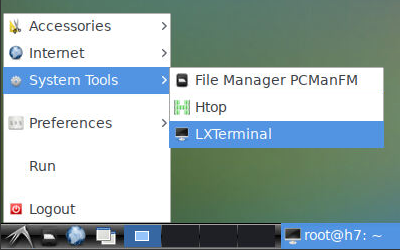
\includegraphics[scale=2.0]{img/terminal}
    \end{figure}

    Enable PIM multicast routing in all the routers (see \autoref{sec:config-router}). 
    \begin{lstlisting}[language={cisco}, emph={ethernet0_ip, ethernet1_ip}]
configure terminal
    ip multicast-routing
    interface f0/0
        ip address 128.238.61.1 255.255.255.0
        ip pim dense-mode
        no shutdown
        exit
    interface f0/1
        ip address 128.238.62.1 255.255.255.0
        ip pim dense-mode
        no shutdown
        exit
    end
    \end{lstlisting}

\section{** Multicast Real-Time Video}
    Start \lstinline{vlc} on \textit{h0} and \textit{h1}:
    \begin{figure}[H]
        \centering
        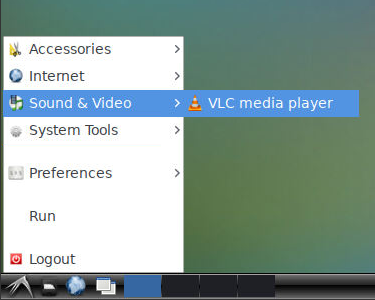
\includegraphics[scale=2.0]{img/vlc-open}
    \end{figure}

    On \textit{h0} \lstinline{vlc}, go to \textit{Tools} menu and select \textit{Preferences}.
    \begin{figure}[H]
        \centering
        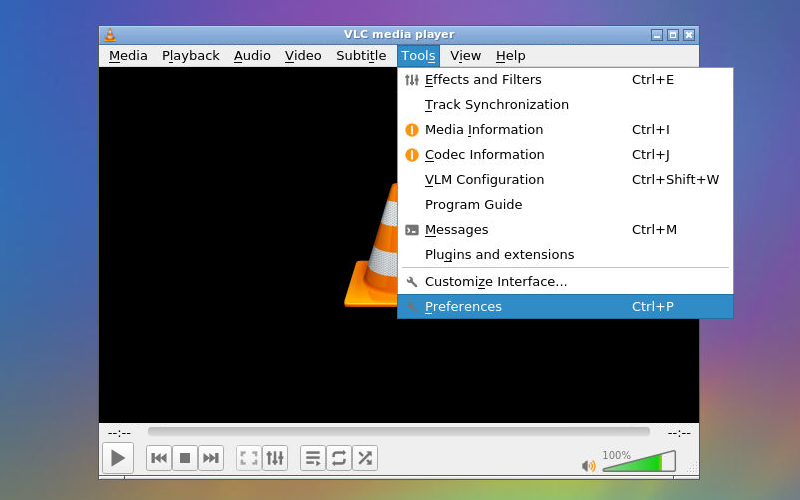
\includegraphics[scale=2]{img/open-pref}
    \end{figure}
    Select \textit{All} for \textit{Show Settings} from the bottom-left corner,
    and search for \texttt{TTL}.
    Select \textit{RTP},
    and enter \texttt{16} for \textit{Hop Limit (TTL)}.
    \begin{figure}[H]
        \centering
        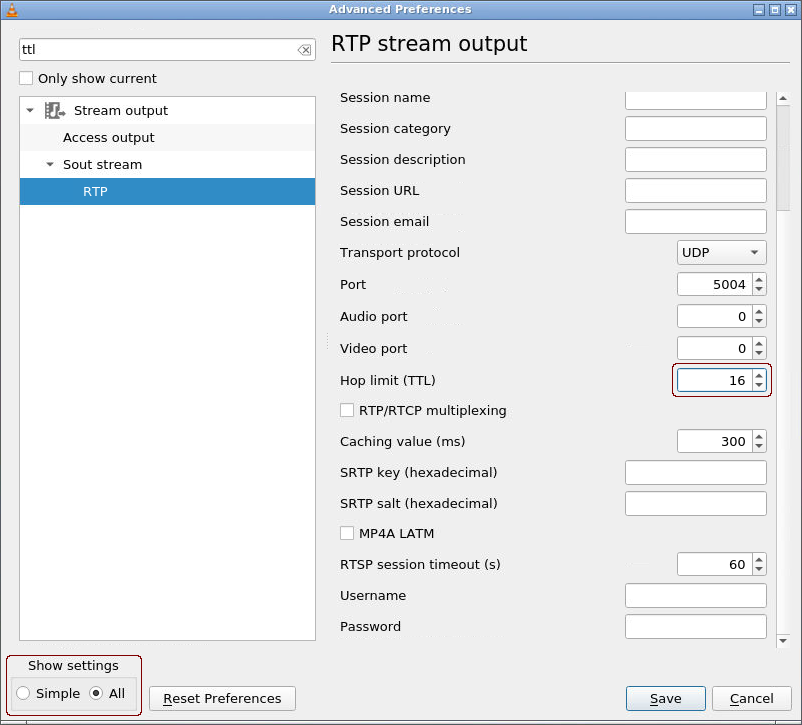
\includegraphics[scale=2.2]{img/pref}
    \end{figure}

    Then, go to the \textit{Media} menu and select \textit{Stream\ldots}.
    \begin{figure}[H]
        \centering
        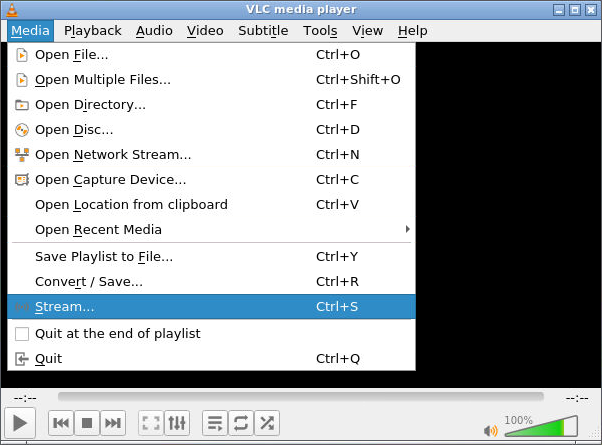
\includegraphics[scale=1.8]{img/open-stream}
    \end{figure}
    Click \textit{Add}. Choose video file \path{/home/netlab/group.mp4} and press \textit{stream} button.
    \begin{figure}[H]
        \centering
        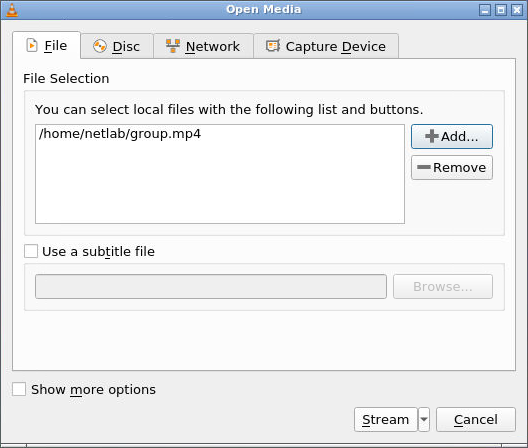
\includegraphics[scale=1.8]{img/stream}
    \end{figure}
    Click \textit{Next}.
    Select \textit{RTP / MPEG Transport Stream} as \textit{New destination} and
    click \textit{Add}.
    \begin{figure}[H]
        \centering
        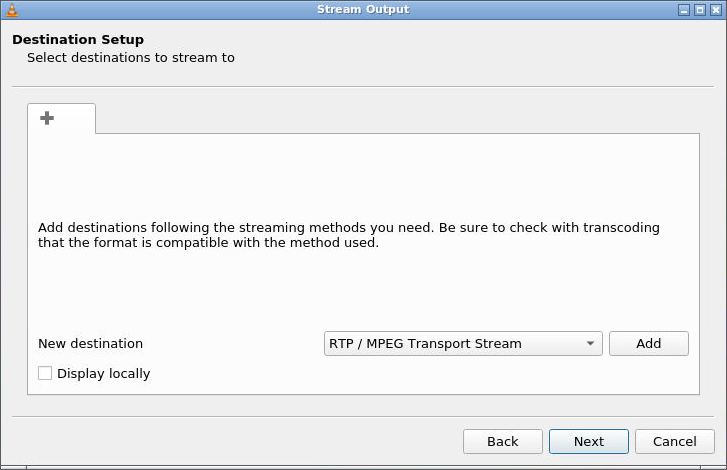
\includegraphics[scale=1.8]{img/stream2}
    \end{figure}
    In the next window, specify the multicast group address to be {224.123.111.101}, with port number {22224}.
    click the \textit{Next} button.
    \begin{figure}[H]
        \centering
        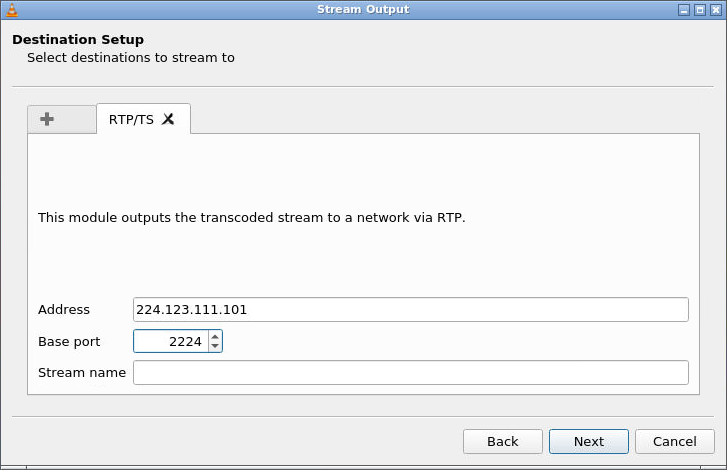
\includegraphics[scale=1.8]{img/stream3}
    \end{figure}
    click the \textit{Next} button again.
    \begin{figure}[H]
        \centering
        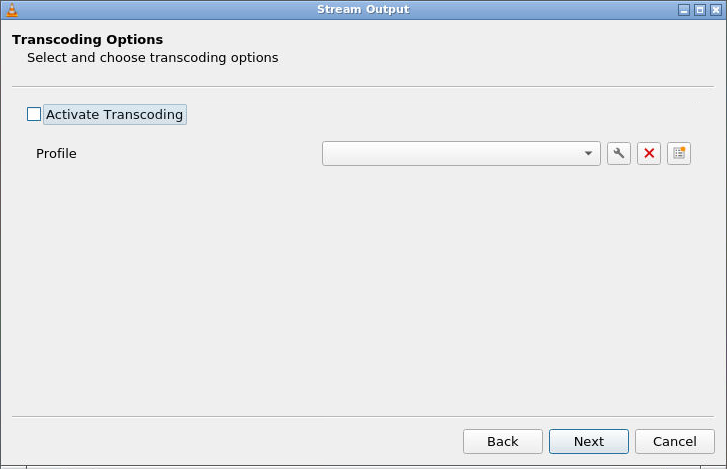
\includegraphics[scale=1.7]{img/stream4}
    \end{figure}
    Then click the \textit{Stream} button.
    \begin{figure}[H]
        \centering
        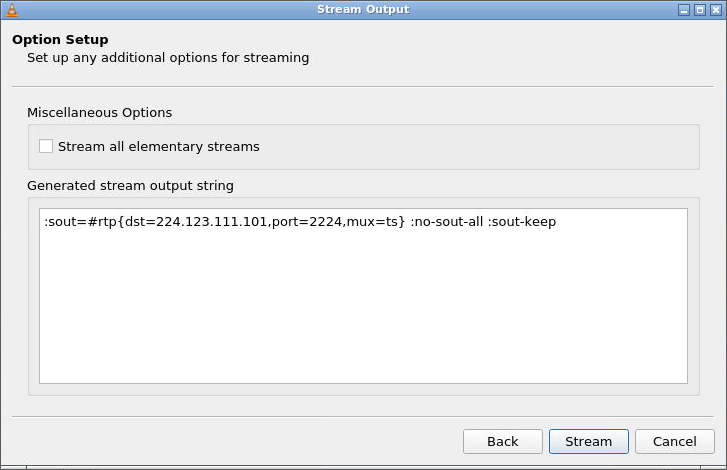
\includegraphics[scale=1.7]{img/stream5}
    \end{figure}
    Now the \lstinline{vlc} on \textit{h0} is transmitting the video clip using \textit{RTP/RTSP/UDP/IP} to the multicast group {224.123.111.101} on port {22224}. 

    On \textit{h1} \lstinline{vlc},
    go to the \textit{Media} menu and select \textit{Open Network Stream\ldots}.
    \begin{figure}[H]
        \centering
        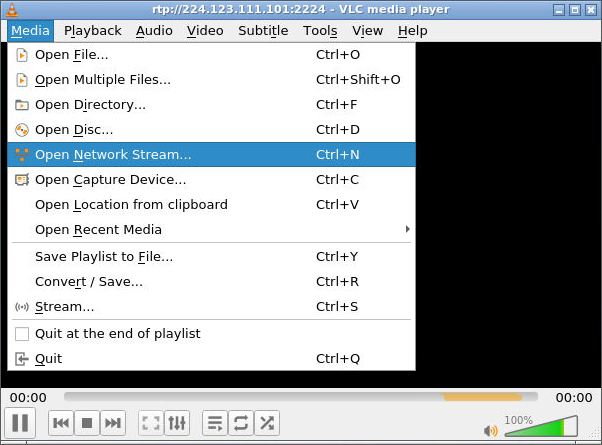
\includegraphics[scale=1.8]{img/open-network}
    \end{figure}
    Enter \texttt{rtp://@224.123.111.101:2224}.
    click the \textit{Play} button.
    \begin{figure}[H]
        \centering
        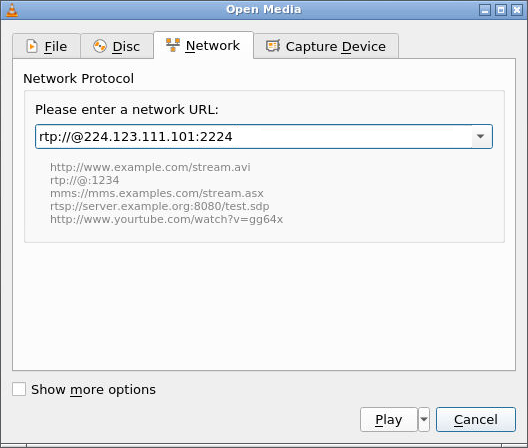
\includegraphics[scale=1.9]{img/network}
    \end{figure}

    Now you should see the received video is displayed on the screen.

    You can do the same on the \textit{h2}, too.


    Execute \lstinline{tcpdump ip multicast} or \lstinline{wireshark} in one console to capture the multicast datagrams.
    In another console, execute \lstinline{tcpdump ip multicast} to monitor the capture process.
    When you see some \texttt{RTCP} packets in the second \lstinline{tcpdump} output, terminate both \lstinline{tcpdump} programs. 

    \begin{report}
    \item Analyze the header format of a \texttt{RTP} data packet and a \texttt{RTCP} Sender (or Receiver) Report packet.
    \end{report}

\clearpage
\begin{appendices}

\section{Configuring a Multicast Router}
    The \lstinline[language={cisco}]{no} form of this command cancels the group membership.
    \begin{subappendices}
\subsection{Configuring IGMP}
    \begin{lstlisting}[language={cisco}, emph={group-address, new-value-in-seconds}]
R1(config)# ip igmp join-group group-address
R1(config)# no ip igmp join-group group-address
R1(config)# ip igmp query-interval new-value-in-seconds
R1(config)# no ip igmp query-interval
show ip igmp groups     ! Displays the multicast groups in the attached networks.
show ip igmp interface  ! Displays multicast related information on a router interface.
debug ip igmp           ! Displays IGMP packets received and transmitted.
    \end{lstlisting}

\subsection{Configuring Multicast Routing}
    \begin{lstlisting}[language={cisco}]
R1(config)# ip multicast-routing
R1(config)# no ip multicast-routing
R1(config)# ip pim [dense-mode | sparse-mode | dense-sparse-mode].
show ip mroute          ! Displays the multicast routing table.
show ip mroute summary  ! Displays a one-line summary for each entry in the multicast routing table.
show ip mroute count    ! Displays multicast statistics.
show ip dvmrp route     ! Displays the DVMRP routing table.
show ip pim neighbor    ! Lists PIM neighbors discovered by the router.
show ip pim interface   ! Displays router interface configurations.
    \end{lstlisting}

\subsection{Cisco~IOS Multicast Diagnostic Tools}
\begin{lstlisting}[language={cisco}]
mtrace
mrinfo
mstat
ping
\end{lstlisting}
    
    \end{subappendices}
\end{appendices}


\end{document}